\subsection{
  Replies to comments received from Jan Sobczyk - Jan. 03, 2013 }

\begin{enumerate}

%........................................................................................................
\vspace{5 mm}
\item
{\em
  ``The meaning of 6 FSI systematics parameters is rather unclear. The
    table 8 is not very helpful in this respect. Also, two out of 6
    parameters (\#0 and \#4) seem to play to role at all, so the motivation
    to have them at all should be better explained.''
}\\
\\
All 6 systematic parameters are {\em normalization factors} for given single $\mu$-like ring event
reconstructed energy spectrum components and,
in some cases, for different energy ranges.
Correlations between these 6 parameters are taken into account.
The FSI+SI error matrix was computed as stated in the first three paragraphs of Sec. 3.1.4.

We think that Table 8 is, in fact, very helpful as it defines exactly
the spectrum components and reconstructed energy ranges to which the different
normalization factors are applied.
For example, $f_{0}^{FSI}$ is a normalization factor for $\nu_{\mu}$ and $\bar{\nu_{\mu}}$ CCQE
in the reconstruted energy range 0 - 0.4 GeV.

The choice of the 6 FSI+SI parameters is well motivated
and it matches the selection of SuperK efficiency parameters (see Sec.\ 3.1.1).
Other parameter choices were attempted, with finer granularity in the
spectrum components and with finer energy binning, but the results were not satisfactory.
For the selected granularity level, these 6 parameters, span {\em all} components 
($\nu_{\mu}$ and $\bar{\nu_{\mu}}$ CCQE, $\nu_{\mu}$ and $\bar{\nu_{\mu}}$ CCnonQE, 
$\nu_{e}$ and $\bar{\nu_{e}}$ CC, NC) and the complete energy range.

Indeed, the effect of $f_{0}^{FSI}$ is negligible (as shown in Fig. 203)  
as there are not many $\nu_{\mu}$ and $\bar{\nu_{\mu}}$ CCQE events below 0.4 GeV
and, in addition, the corresponding element of the error matrix (Fig. 17) is very small.
The effect of $f_{4}^{FSI}$ is also negligible (as shown in Fig. 207) as there are not many 
$\nu_{e}$ and $\bar{\nu_{e}}$ CC events in the single $\mu$-like ring spectrum.
Simililarly, other systematic parameters included in this analysis have a negligible
effect (see, for example, the $\nu_{e}$ SuperK efficiency error, Fig. 168).
We think it is proper to implement all these nuisance parameters in the
single $\mu$-like ring event reconstructed energy spectrum p.d.f.
They parameterize uncertainties which exist and have been evaluated 
and this is sufficient enough motivation.
By implementing these nuisance parameters we can explicitly check
their effect on the oscillation parameter measurement.
However, as mentioned in various places in the main text,
we do not think it is necessary to include all nuisance parameters
in the oscillation fit.

%........................................................................................................
\vspace{5 mm}
\item
{\em
   ``A choice of 8 most relevant systematics is not completely clear.
   For example, the Table 11 suggests that mising $f_{20}$ is more important
   than some other which were actually selected.''
}\\
\\
We think the method used for choosing the most important systematics is clear but,
on reflection, Table 11 is misleading.

We have studied how the oscillation parameters are shifted, as a result of varying systematic parameters,
at {\em many different} points in the oscillation parameter space.
The chosen grid is shown in Appendix G.
The systematic parameters we consider to be ``important'' are those which can shift the value of an oscillation
parameter, in at least one of the points considered, by more than 25\% of the expected statistical error 
at that same point.

Although $f_{20}^{banff}$ appears to be causing, in absolute terms, 
a larger shift in the oscillation parameters
than some of the selected systematic parameters,
its effect is still smaller than 
25\% of the expected statistical error at the point where this shift occurs.

In version 2 of T2K-TN-141, Table 11 will be modified so that, 
rather than showing the maximum oscillation parameter shifts,
it shows the maximum shift relative to the expected statistical error
computed at the point where the maximum shift occurs.

We hope that the above comments, and the revised Table to appear in version 2, clarify the issue.
In summary, the criterion for choosing the most important systematics is clear and robust,
and no exception was made to that criterion. Systematic parameter $f_{20}^{banff}$ does not meet
our selection criterion. It is clear than many variations to that selection criterion are possible.
However, the small number of parameters yielded by our choice (8 out of 48) and the fact that the 
`2+8' and `2+N' contours are nearly identical justifies our choice.

%........................................................................................................
\vspace{5 mm}
\item
{\em
  ``In Figs 41, 43 the data points seem to be (on average) slightly
    above the red curve. This is probably because in one of the $E_{rec}$ bins
    (around 0.8 GeV) the number of events is zero and this point is not
    shown?... If it is so, perhaps it would be useful to have this point
    on the figures?''
}\\
\\
Indeed, one of the bins (0.8 - 0.9 GeV) has no events in it.
In version 2 of T2K-TN-141, data points are shown for bins with 0 events in all plots.

%........................................................................................................
\vspace{5 mm}
\item
{\em
  ``I have some problems in understanding structures that appear in
    Figs. 161 - 256.  In particular in: 172, 173, 185, 186, 190, 192, 193,
    194, 196, 197, 206. Do you have some intuition to explain these
    sometimes rather bizarre shapes?''
}\\
\\
The features of these plots are understood (and validated by cross-comparing them with 
the KIT analysis) but they are not always easy to explain simply.

Each of Figs. 172, 173, 185, 186, 190, 192, 193, 194, 196, 197 and 206
shows the effects of $\pm$1$\sigma$ and $\pm$3$\sigma$ variations
of a given systematic parameter on the 
single $\mu$-like ring event reconstructed energy spectrum 
expected under the {\em no oscillation} hypothesis (all 3 mixing angles set to 0).
\begin{itemize}
\item
Fig. 172 shows the effect of $f_{3}^{banff}$ ($\nu_{\mu}$ flux normalization in the 0.6 - 0.7 GeV true energy range)
\item
Fig. 173 shows the effect of $f_{4}^{banff}$ ($\nu_{\mu}$ flux normalization in the 0.7 - 1.0 GeV true energy range)
\item
Fig. 185 shows the effect of $f_{16}^{banff}$ (CCQE axial mass)
\item
Fig. 186 shows the effect of $f_{17}^{banff}$ (resonance neutrino-production axial mass)
\item
Fig. 190 shows the effect of $f_{21}^{banff}$ (CC1$\pi$ normalization in the 0 - 2.5 GeV true energy range)
\item
Fig. 192 shows the effect of $f_{pF}$
\item
Fig. 193 shows the effect of $f_{SF}$
\item
Fig. 194 shows the effect of $f_{Wshape}$
\item
Fig. 196 shows the effect of $f_{\pi-less\Delta}$
\item
Fig. 197 shows the effect of $f_{bindE}$
\item
Fig. 206 shows the effect of $f_{3}^{FSI}$ ($\nu_{\mu}$ and $\bar{\nu_{\mu}}$ CCnonQE normalization)
\end{itemize}

To understand these plots, one needs to 
consider which spectrum components are affected by each systematic parameter, 
the reconstructed energy spectrum of these components and the range of 
true energy bins that contributes to each reconstructed energy bin.
For example, in Fig.\ \ref{fig:jan_fig172_features}
we show the single $\mu$-like ring event reconstructed energy spectrum,
the contribution to that spectrum from all true $\nu_\mu$ interactions and
the contribution to that spectrum from true $\nu_\mu$ interactions with true neutrino
energy in the range 0.6 - 0.7 GeV. The fractional contribution to the spectrum
from true $\nu_\mu$ interactions with true neutrino
energy in the 0.6 - 0.7 GeV range is also shown in the right plot.
From these plots, it is straightforward to see the origin of the structure seen in Fig.\ 172
in T2K-TN-141v1, which shows the effect of tweaking the 
$\nu_{\mu}$ flux normalization in the true energy range 0.6 - 0.7 GeV.
Similar comments apply to Figs. 173, 185, 186, 190 and 206,
though in some cases, unlike in the simple example mentioned above, 
an additional complication arises from the  fact that
the size of the systematic variation has a functional dependence on the reconstructed and/or true energy.

The structure seen in Figs 192, 193 and 197 can also be understood considering that
such changes to the nuclear model shift the reconstructed energy spectrum either towards
higher or lower energies.

%{\color{red} anything else we could add to explain the features?}

\begin{figure*}[htb]
\begin{minipage}[t]{0.48\linewidth}
\center
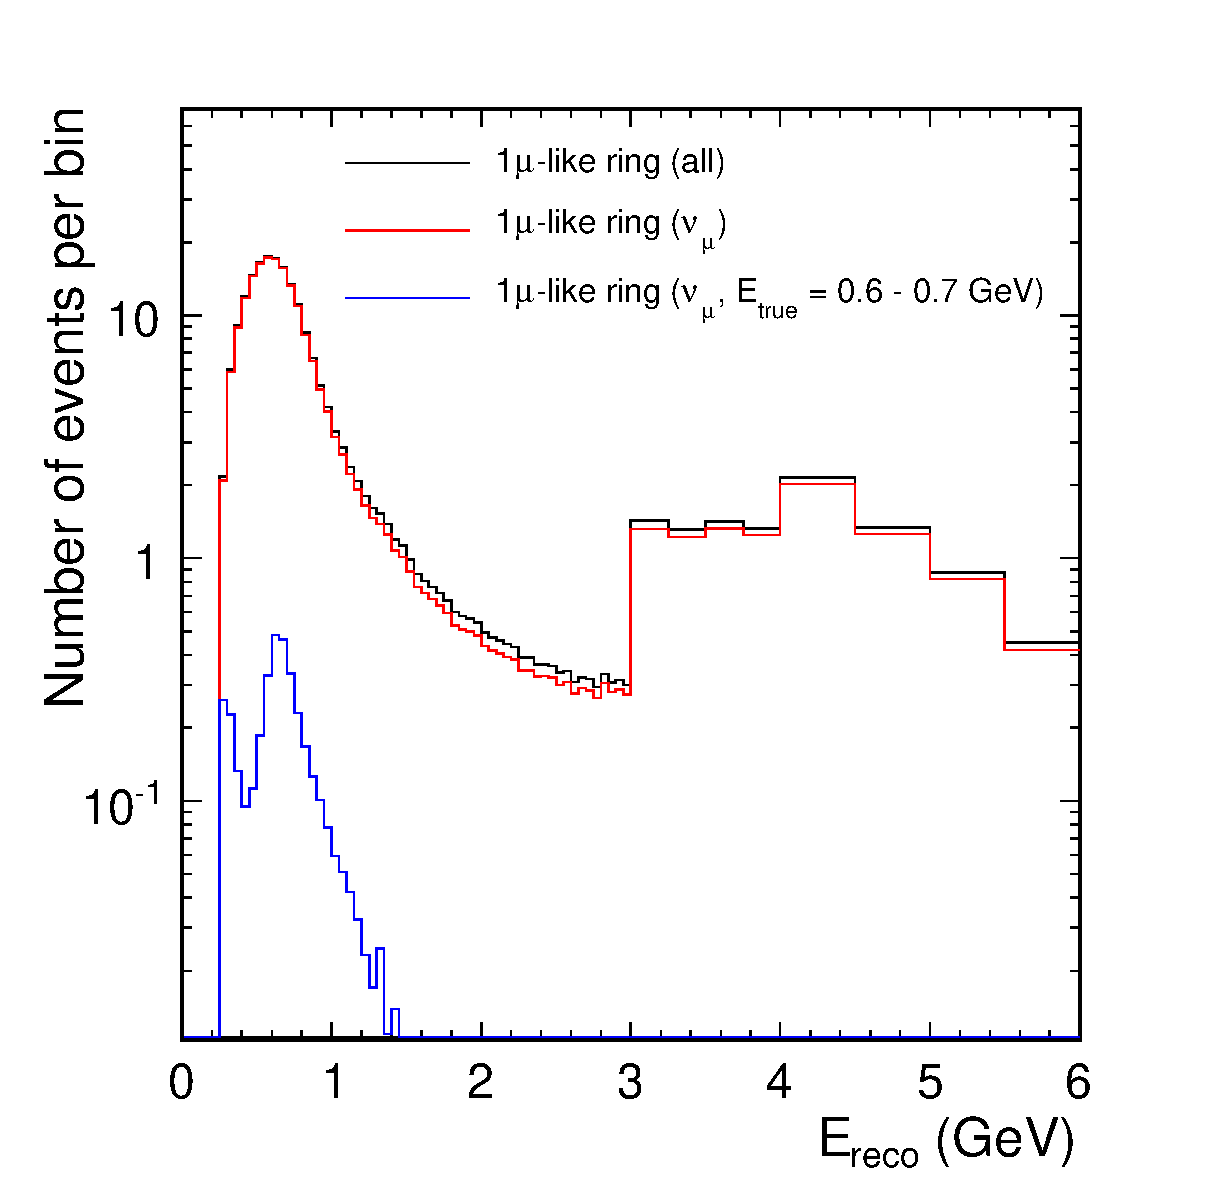
\includegraphics[width=20pc]{./images/jan_fig172features_spectra.eps}
%\caption {
%  Systematic parameter pulls for the `2+8' fit to the Run 1+2 dataset.
%}
%\label{fig:results_data12_pulls}
\end{minipage}
\hspace{0.06\linewidth}
\begin{minipage}[t]{0.48\linewidth}
\center
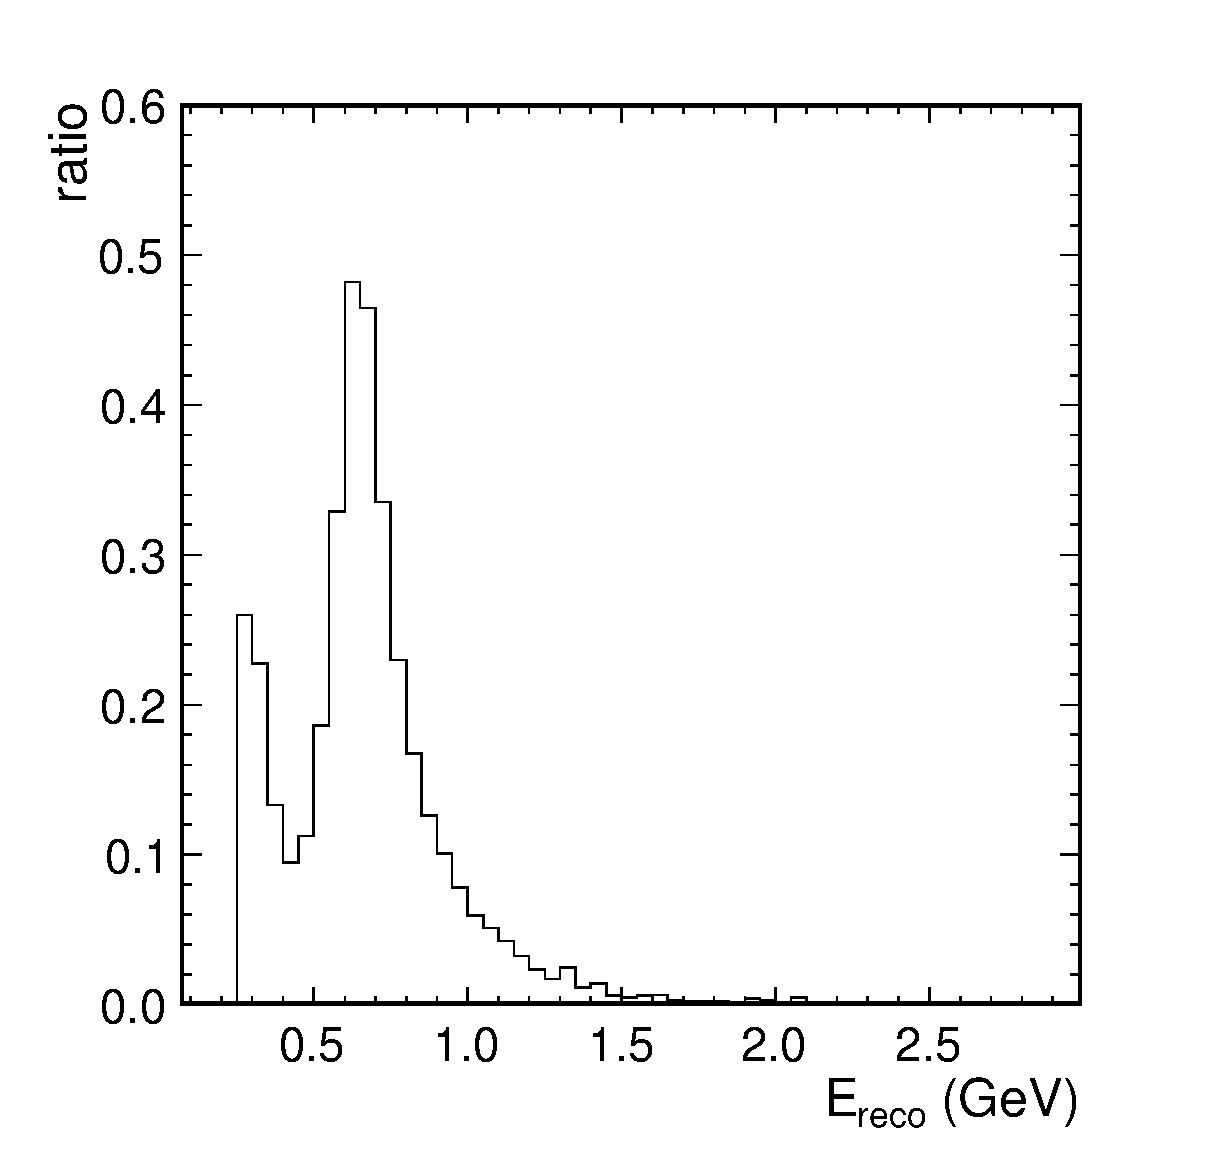
\includegraphics[width=20pc]{./images/jan_fig172features_ratio.eps}
\end{minipage}
\caption {
 Single $\mu$-like ring reconstructed energy spectrum and contributions to it from all true 
 $\nu_{\mu}$ interactions and from true $\nu_{\mu}$ interactions with true energy in the range
 0.6 - 0.7 GeV (left) and the fractional contribution to the reconstructed energy spectrum 
 from true $\nu_{\mu}$ interactions with true energy in the range 0.6 - 0.7 GeV (right) 
}
\label{fig:jan_fig172_features}
\end{figure*}


%........................................................................................................
\vspace{5 mm}
\item
{\em
  ``In Fig. 23 (and many others) you show only "one-direction" changes
    introduced by 1sigma variations of systematics i.e. variations for
    either plus or minus sigma. What about the other sign? I understand
    that if you add this information the figures become difficult to read?
    Anyhow, it would be interesting to see some examples.''
}\\
\\
In fact, the effect of both $\pm$1$\sigma$ variation is shown in these plots.
For example, in Fig.\ 23 mentioned in your question, we vary 8 systematics
and more than 8 arrows can be seen. There are 16 arrows in total (8 systematic
parameters $\times$ 2 parameter variations),
although not all 16 can be seen clearly. Please see Fig.\ 26 in which these arrows 
can be seen more clearly.

%\begin{figure*}[htb]
%\begin{minipage}[t]{0.48\linewidth}
%\center
%\includegraphics[width=20pc]{{./images/important-0.900000-0.002400_testbig_minus}.eps}
%%\caption {
%%  Systematic parameter pulls for the `2+8' fit to the Run 1+2 dataset.
%%}
%%\label{fig:results_data12_pulls}
%\end{minipage}
%\hspace{0.06\linewidth}
%\begin{minipage}[t]{0.48\linewidth}
%\center
%\includegraphics[width=20pc]{{./images/important-0.900000-0.002400_testbig_plus}.eps}
%\end{minipage}
%\caption {  
%  Effects of variation by $-1\sigma$ (left) and $+1\sigma$ (right) of the 8 dominant systematic parameters
%  on the oscillation parameters $\sin^{2}2\theta_{23}$ and $\Delta m^{2}_{32}$.
%  The ellipse shown is one quarter the size of the statistical error. 
%  The true 23-sector oscillation parameters used are 
%  $\sin^{2}2\theta_{23}$ = 0.90 and $\Delta m^{2}_{32}$ = 2.4$\times10^{-3} eV^{2}/c^{4}$.
%  The 2012 PDG values are used for $\sin^{2}2\theta_{13}$, $\sin^{2}2\theta_{12}$ and $\Delta m^{2}_{21}$,
%  and $\delta_{CP}$=0. The normal mass hierarchy is assumed.
%}
%\label{fig:jan_fig172_features}
%\end{figure*}
%
%{\color{red} Tom: I'm not sure I like these plots. I thought it'd be
%  good to put but they are dramatic, and not intuitive (why -sigma
%  have such a small effect)
%  maybe it's best to just be implicit (i.e. no plots)? }
%

\end{enumerate}
